
%%%%%%%%%%%%%%%%%%%%%%%%%%%%%%%%%%%%%%%%%%%%%%%%%%%%%%%%
%
% Copyright (c) 2003-2009 by University of Queensland
% Earth Systems Science Computational Center (ESSCC)
% http://www.uq.edu.au/esscc
%
% Primary Business: Queensland, Australia
% Licensed under the Open Software License version 3.0
% http://www.opensource.org/licenses/osl-3.0.php
%
%%%%%%%%%%%%%%%%%%%%%%%%%%%%%%%%%%%%%%%%%%%%%%%%%%%%%%%%


\section{3-D Wave Propagation}
\label{WAVE CHAP}

In this next example we want to calculate the displacement field $u\hackscore{i}$ for any time $t>0$ by solving the wave equation:
\index{wave equation}
\begin{eqnarray}\label{WAVE general problem}
\rho u\hackscore{i,tt} - \sigma\hackscore{ij,j}=0
\end{eqnarray}
in a three dimensional block of length $L$ in $x\hackscore{0}$
and $x\hackscore{1}$ direction and height $H$
in $x\hackscore{2}$ direction. $\rho$ is the known density which may be a function of its location.
$\sigma\hackscore{ij}$ is the stress field \index{stress} which in case of an isotropic, linear elastic material is given by
\begin{eqnarray} \label{WAVE stress}
\sigma\hackscore{ij} & = & \lambda u\hackscore{k,k} \delta\hackscore{ij} + \mu ( u\hackscore{i,j} + u\hackscore{j,i})
\end{eqnarray}
where $\lambda$ and $\mu$ are the Lame coefficients 
\index{Lame coefficients} and $\delta\hackscore{ij}$ denotes the Kronecker symbol\index{Kronecker symbol}.
On the boundary the normal stress is given by
\begin{eqnarray} \label{WAVE natural}
\sigma\hackscore{ij}n\hackscore{j}=0
\end{eqnarray}
for all time $t>0$.

\begin{figure}[t!]
\centerline{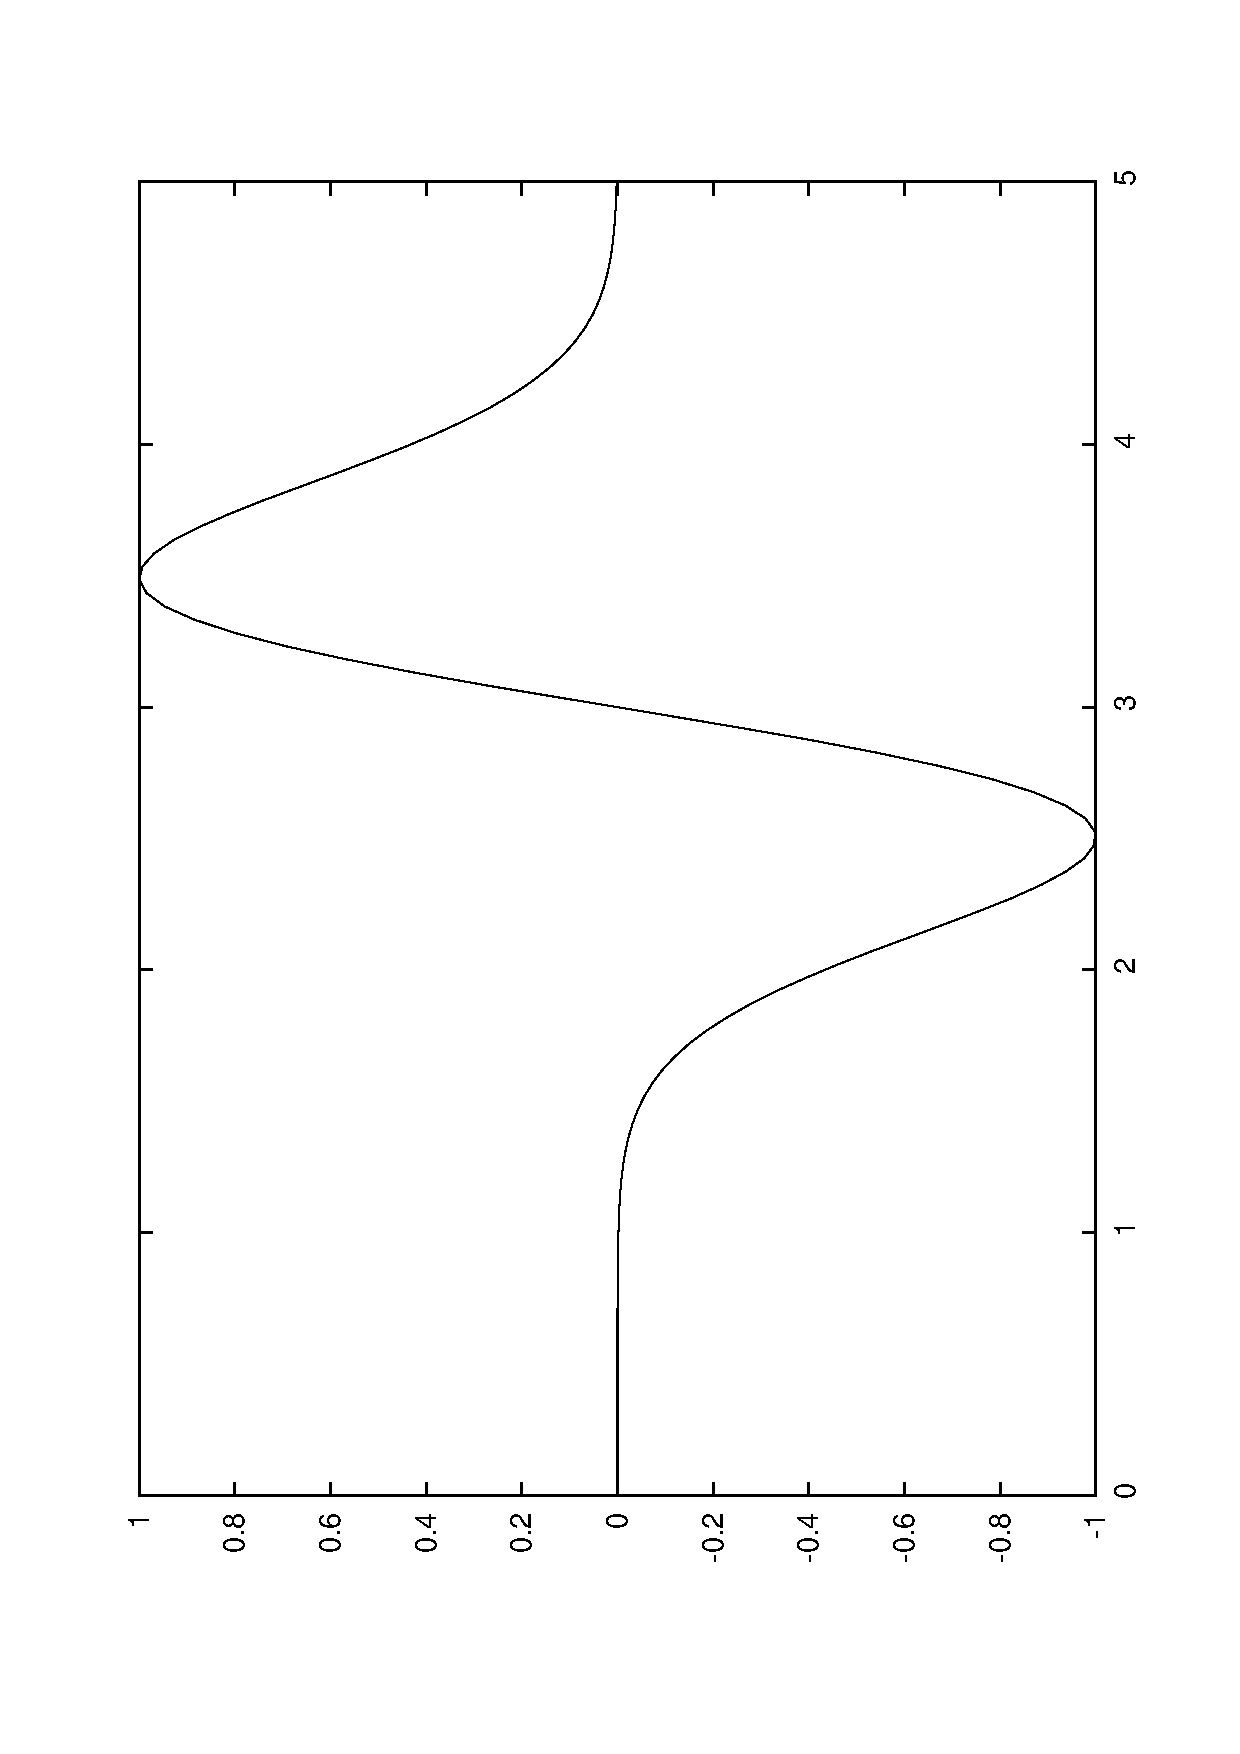
\includegraphics[angle=-90,width=4.in]{figures/waveu}}
\caption{Input Displacement at Source Point ($\alpha=0.7$, $t\hackscore{0}=3$, $U\hackscore{0}=1$).}
\label{WAVE FIG 1.2}
\end{figure}

\begin{figure}[t!]
\centerline{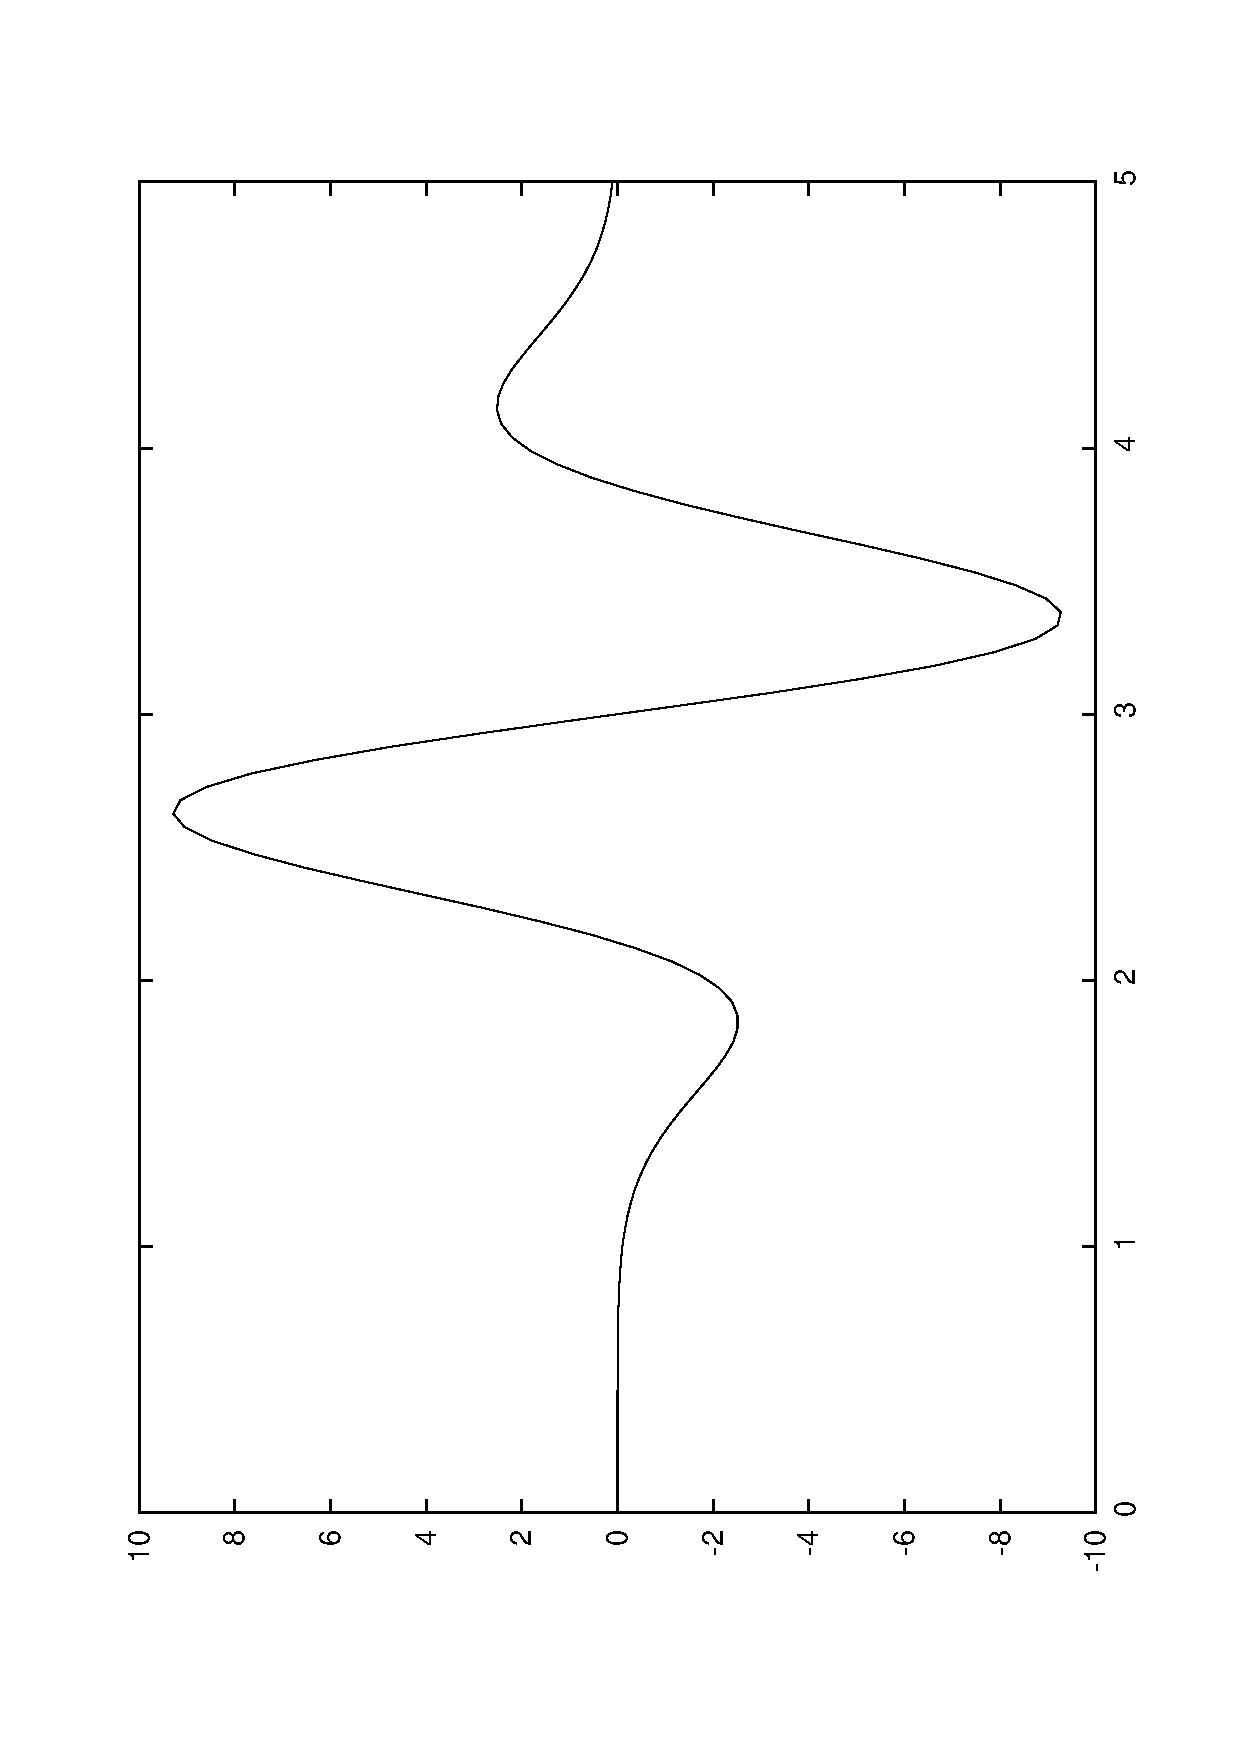
\includegraphics[angle=-90,width=4.in]{figures/wavea}}
\caption{Input Acceleration at Source Point ($\alpha=0.7$, $t\hackscore{0}=3$, $U\hackscore{0}=1$).}
\label{WAVE FIG 1.1}
\end{figure}

Here we are modelling a point source at the point $x\hackscore C$ in the $x\hackscore{0}$-direction
which is a negative pulse of amplitude $U\hackscore{0}$ followed by the same 
positive pulse. In mathematical terms we use
\begin{eqnarray} \label{WAVE source}
u\hackscore{0}(x\hackscore C,t)= U\hackscore{0} \; \sqrt{2}  \frac{(t-t\hackscore{0})}{\alpha} e^{\frac{1}{2}-\frac{(t-t\hackscore{0})^2}{\alpha^2}} \ 
\end{eqnarray}
for all $t\ge0$ where $\alpha$ is the width of the pulse and $t\hackscore{0}$ is the time when
the pulse changes from negative to positive. In the simulations we will choose $\alpha=0.3$ and $t\hackscore{0}=2$, see Figure~\ref{WAVE FIG 1.2}
and will apply the source as a constraint in a in a sphere of small radius around the point
$x\hackscore C$.  

 We use an explicit time integration scheme to calculate the displacement field $u$ at 
certain time marks $t^{(n)}$ where $t^{(n)}=t^{(n-1)}+h$ with time step size $h>0$. In the following the upper index ${(n)}$ refers to values at time $t^{(n)}$. We use the Verlet scheme \index{Verlet scheme} with constant time step size $h$
which is defined by
\begin{eqnarray} \label{WAVE dyn 2}
u^{(n)}=2u^{(n-1)}-u^{(n-2)} + h^2 a^{(n)} \\
\end{eqnarray}
for all $n=2,3,\ldots$. It is designed to solve a system of equations of the form
\begin{eqnarray} \label{WAVE dyn 2b} 
u\hackscore{,tt}=G(u)
\end{eqnarray}
where one sets $a^{(n)}=G(u^{(n-1)})$.

In our case $a^{(n)}$ is given by
\begin{eqnarray}\label{WAVE dyn 3}
\rho a^{(n)}\hackscore{i}=\sigma^{(n-1)}\hackscore{ij,j}
\end{eqnarray}
and boundary conditions
\begin{eqnarray} \label{WAVE natural at n}
\sigma^{(n-1)}\hackscore{ij}n\hackscore{j}=0
\end{eqnarray}
derived from \eqn{WAVE natural} where 
\begin{eqnarray} \label{WAVE dyn 3a}
\sigma\hackscore{ij}^{(n-1)} & = & \lambda u^{(n-1)}\hackscore{k,k} \delta\hackscore{ij} + \mu ( u^{(n-1)}\hackscore{i,j} + u^{(n-1)}\hackscore{j,i}).
\end{eqnarray}
We also need to apply the constraint 
\begin{eqnarray} \label{WAVE dyn 3aa}
a^{(n)}\hackscore{0}(x\hackscore C,t)= U\hackscore{0} 
\frac{\sqrt(2.)}{\alpha^2} (4\frac{(t-t\hackscore{0})^3}{\alpha^3}-6\frac{t-t\hackscore{0}}{\alpha})e^{\frac{1}{2}-\frac{(t-t\hackscore{0})^2}{\alpha^2}}
\end{eqnarray}
which is derived from equation~\ref{WAVE source} by calculating the second order time derivative,
see Figure~\ref{WAVE FIG 1.1}. Now we have converted our problem for displacement, $u^{(n)}$, into a problem for 
acceleration, $a^{(n)}$, which now depends 
on the solution at the previous two time steps, $u^{(n-1)}$  and $u^{(n-2)}$.

In each time step we have to solve this problem to get the acceleration $a^{(n)}$, and we will
use the \LinearPDE class of the \linearPDEs to do so. The general form of the PDE defined through
the \LinearPDE class is discussed in \Sec{SEC LinearPDE}. The form which is relevant here is
\begin{equation}\label{WAVE dyn 100}
D\hackscore{ij} a^{(n)}\hackscore{j} = - X\hackscore{ij,j}\; .
\end{equation}
The natural boundary condition
\begin{equation}\label{WAVE dyn 101}
n\hackscore{j}X\hackscore{ij} =0 
\end{equation}
is used. 
With $u=a^{(n)}$ we can identify the values to be assigned to $D$ and $X$:
\begin{equation}\label{WAVE  dyn 6}
\begin{array}{ll}
D\hackscore{ij}=\rho \delta\hackscore{ij}&
X\hackscore{ij}=-\sigma^{(n-1)}\hackscore{ij} \\
\end{array}
\end{equation}
Moreover we need to define the location $r$ where the constraint~\ref{WAVE dyn 3aa} is applied. We will apply
the constraint on a small sphere of radius $R$ around $x\hackscore C$ (we will use 3p.c. of the width of the domain):  
\begin{equation}\label{WAVE  dyn 6 1}
q\hackscore{i}(x) = 
\left\{
\begin{array}{rc}
1 & \|x-x_c\|\le R \\
0 & \mbox{otherwise}
\end{array}
\right.
\end{equation}
The following script defines a the function \function{wavePropagation} which
implements the Verlet scheme to solve our wave propagation problem. 
The argument \var{domain} which is a \Domain class object
defines the domain of the problem. \var{h} and \var{tend} are the time step size
and the end time of the simulation. \var{lam}, \var{mu} and 
\var{rho} are material properties. 
\begin{python}
def wavePropagation(domain,h,tend,lam,mu,rho, x_c, src_radius, U0):
   # lists to collect displacement at point source which is returned to the caller
   ts, u_pc0,u_pc1,u_pc2=[], [], [], []
  
   x=domain.getX()
   # ... open new PDE ...
   mypde=LinearPDE(domain)
   mypde.getSolverOptions().setSolverMethod(mypde.getSolverOptions().LUMPING)
   kronecker=identity(mypde.getDim())
   dunit=numpy.array([1.,0.,0.]) # defines direction of point source
   mypde.setValue(D=kronecker*rho, q=whereNegative(length(x-xc)-src_radius)*dunit)
   # ... set initial values ....
   n=0
   # for first two time steps
   u=Vector(0.,Solution(domain))
   u_last=Vector(0.,Solution(domain))
   t=0
   # define the location of the point source 
   L=Locator(domain,xc)
   # find potential at point source
   u_pc=L.getValue(u)
   print "u at point charge=",u_pc
   # open file to save displacement at point source
   u_pc_data=FileWriter('./data/U_pc.out')
   ts.append(t); u_pc0.append(u_pc[0]), u_pc1.append(u_pc[1]), u_pc2.append(u_pc[2])

   while t<tend:
     t+=h
     # ... get current stress ....
     g=grad(u)
     stress=lam*trace(g)*kronecker+mu*(g+transpose(g))
     # ... get new acceleration ....
     amplitude=U0*(4*(t-t0)**3/alpha**3-6*(t-t0)/alpha)*sqrt(2.)/alpha**2 \
                                             *exp(1./2.-(t-t0)**2/alpha**2)
     mypde.setValue(X=-stress, r=dunit*amplitude)
     a=mypde.getSolution()
     # ... get new displacement ...
     u_new=2*u-u_last+h**2*a
     # ... shift displacements ....
     u_last=u
     u=u_new
     n+=1
     print n,"-th time step t ",t
     u_pc=L.getValue(u)
     print "u at point charge=",u_pc
     # save displacements at point source to file for t > 0
     ts.append(t); u_pc0.append(u_pc[0]), u_pc1.append(u_pc[1]), \
                                                    u_pc2.append(u_pc[2])

     # ... save current acceleration in units of gravity and displacements 
     if n==1 or n%10==0: saveVTK("./data/usoln.%i.vtu"%(n/10), \
                                 acceleration=length(a)/9.81,
                                 displacement = length(u), \
				 tensor = stress, Ux = u[0] )

   return ts, u_pc0, u_pc1, u_pc2
\end{python}
Notice that 
all coefficients of the PDE which are independent of time $t$ are set outside the \code{while} 
loop. This is very efficient since it allows the \LinearPDE class to reuse information as much as possible 
when iterating over time. 

The statement 
\begin{python}
mypde.getSolverOptions().setSolverMethod(mypde.getSolverOptions().LUMPING) 
\end{python}
switches on the use of an aggressive approximation of the PDE operator as a diagonal matrix
formed from the coefficient \var{D}.
The approximation allows, at the cost of 
additional error, very fast 
solution of the PDE. When using lumping the presence of \var{A}, \var{B} or \var{C} will produce wrong results.
 
There are a few new \escript functions in this example: 
\code{grad(u)} returns the gradient $u\hackscore{i,j}$ of $u$ (in fact \var{grad(g)[i,j]}=$=u\hackscore{i,j}$).
There are restrictions on the argument of the \function{grad} function, for instance
the statement \code{grad(grad(u))} will raise an exception.
\code{trace(g)} returns the sum of the main diagonal elements \var{g[k,k]} of \var{g} 
and \code{transpose(g)} returns the matrix transpose of \var{g} (ie. $\var{transpose(g)[i,j]}=\var{g[j,i]}$). 

We initialize the values of \code{u} and \code{u_last} to be zero. It is important
to initialize both with the \SolutionFS \FunctionSpace as they have to be seen as solutions of PDEs from previous time steps. In fact, the \function{grad} does not accept arguments with a certain \FunctionSpace, for more details see \Sec{SEC ESCRIPT DATA}. 

The \class{Locator} is designed to extract values at a given location (in this case $x\hackscore C$) from functions such as the displacement vector \code{u}. Typically the \class{Locator} is used in the following form:  
\begin{python}
L=Locator(domain,xc)
u=...
u_pc=L.getValue(u)
\end{python}
The return value \code{u_pc} is the value of \code{u} at the location \code{xc}\footnote{In fact the finite element node which is closest to the given position. The usage of  \class{Locator} is MPI save.}. The values
are collected in the lists \var{u_pc0}, \var{u_pc1} and \var{u_pc2} together with the 
corresponding time marker in \var{ts}. The values are handed back to the caller. Later we will show to ways to
access these data.

One of the big advantages of the Verlet scheme is the fact that the problem to be solved 
in each time step is very simple and does not involve any spatial derivatives (which is what allows us to use lumping in this simulation).
The problem becomes so simple because we use the stress from the last time step rather then the stress which is
actually present at the current time step. Schemes using this approach are called an explicit time integration 
schemes \index{explicit scheme} \index{time integration!explicit}. The 
backward Euler scheme we have used in \Chap{DIFFUSION CHAP} is 
an example of an implicit scheme
\index{implicit scheme} \index{time integration!implicit}. In this case one uses the actual status of 
each variable at a particular time rather then values from previous time steps. This will lead to a problem which is 
more expensive to solve, in particular for non-linear problems. 
Although 
explicit time integration schemes are cheap to finalize a single time step, they need significantly smaller time
steps then implicit schemes and can suffer from stability problems. Therefore they need a 
very careful selection of the time step size $h$.

An easy, heuristic way of choosing an appropriate
time step size is the Courant condition \index{Courant condition} \index{explicit scheme!Courant condition}
which says that within a time step a information should not travel further than a cell used in the 
discretization scheme. In the case of the wave equation the velocity of a (p-) wave is given as
$\sqrt{\frac{\lambda+2\mu}{\rho}}$ so one should choose $h$ from
\begin{eqnarray}\label{WAVE dyn 66}
h= \frac{1}{5} \sqrt{\frac{\rho}{\lambda+2\mu}} \Delta x
\end{eqnarray}
where $\Delta x$ is the cell diameter. The factor $\frac{1}{5}$ is a safety factor considering the heuristics of 
the formula. 

\begin{figure}[t]
\begin{center}
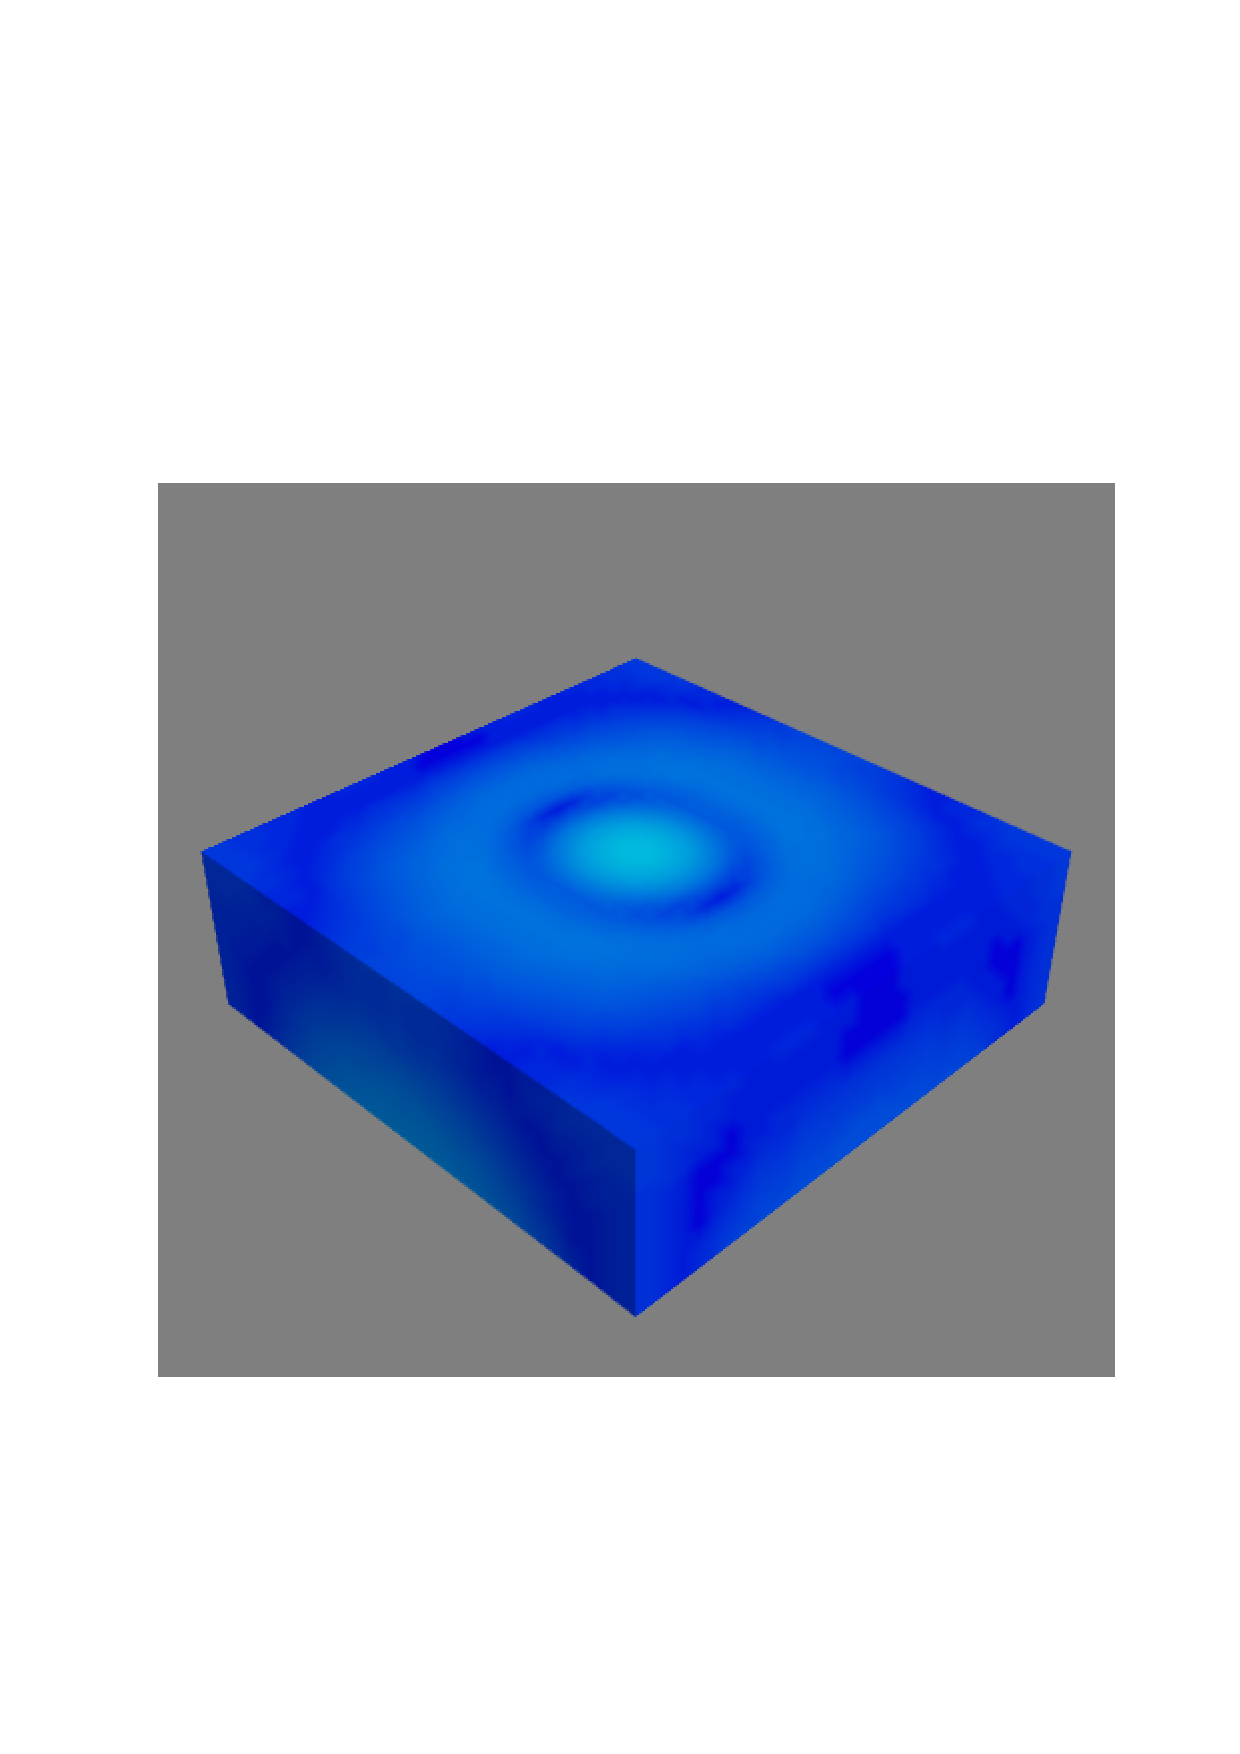
\includegraphics[width=2in]{figures/Wave11}
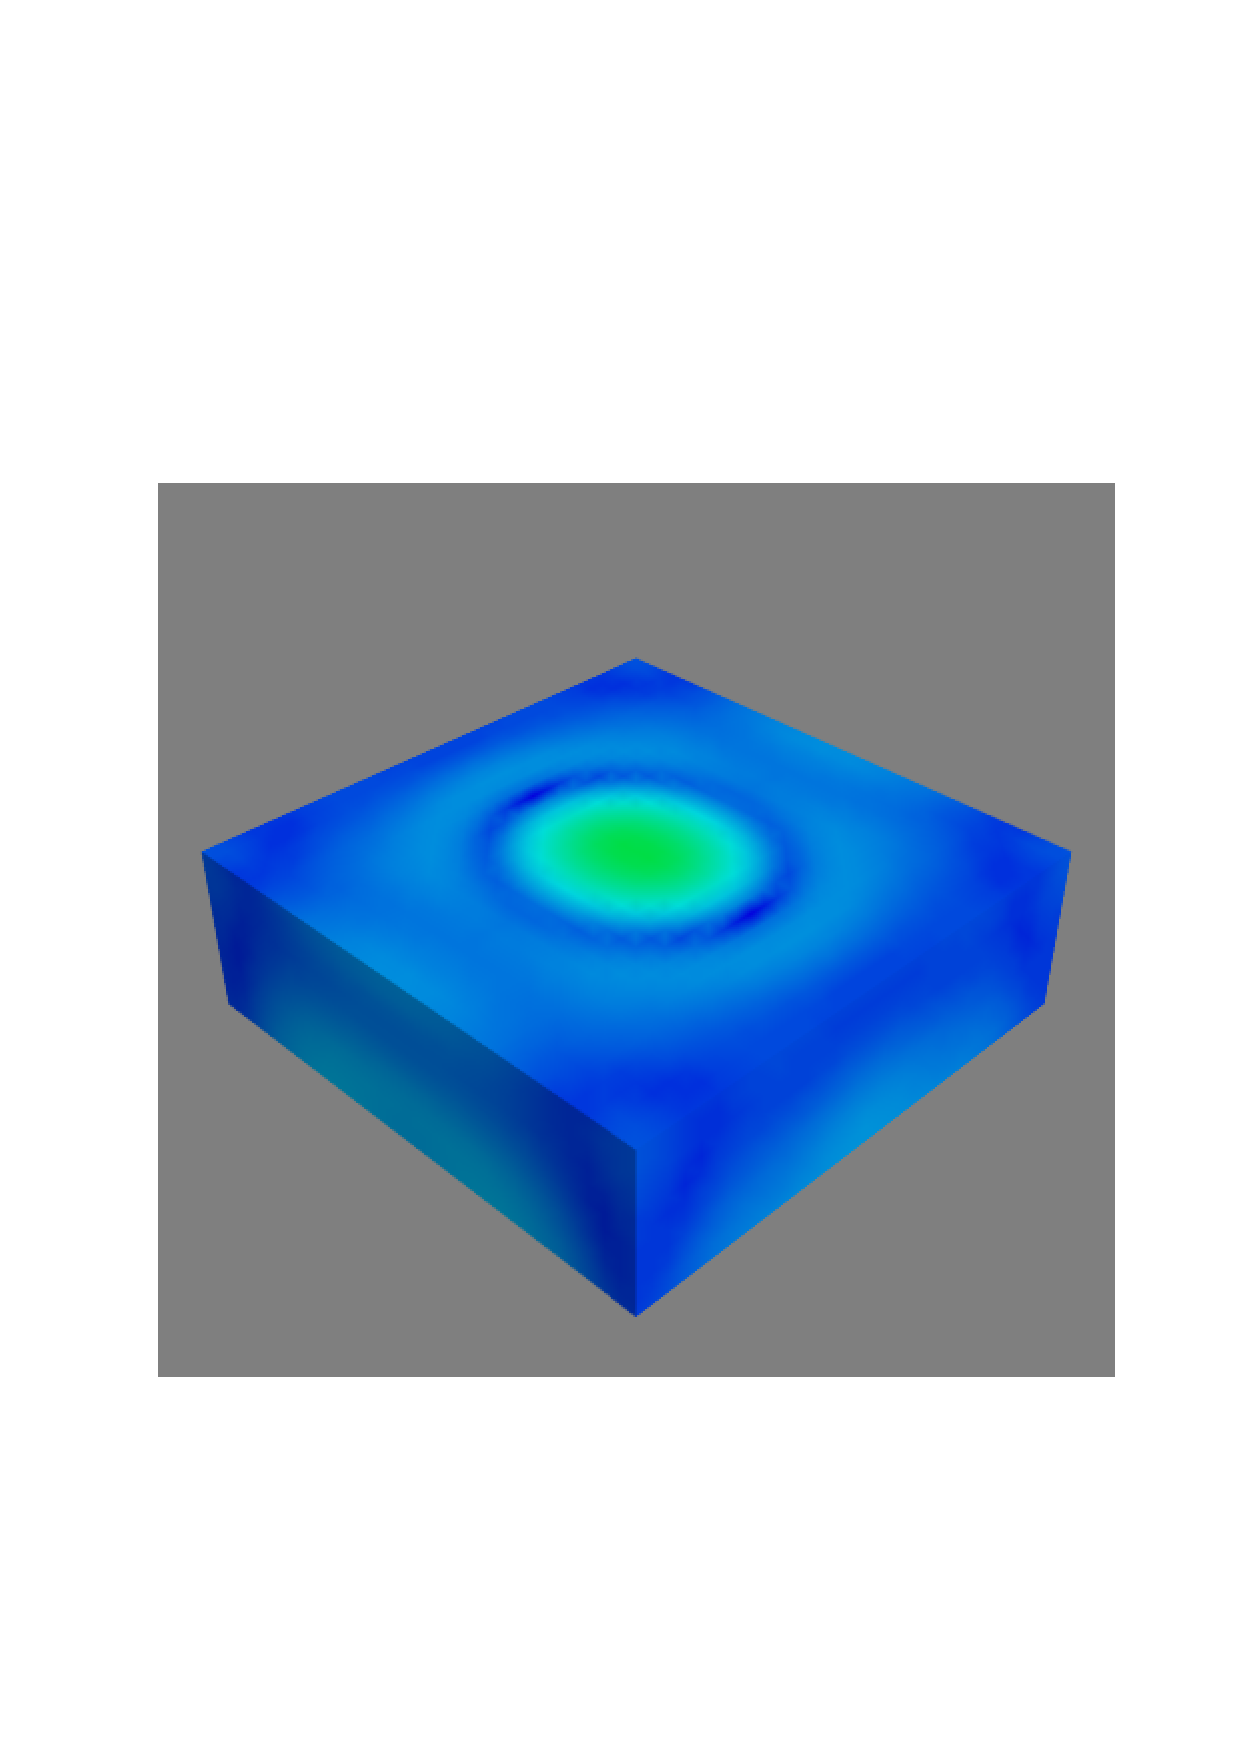
\includegraphics[width=2in]{figures/Wave22}
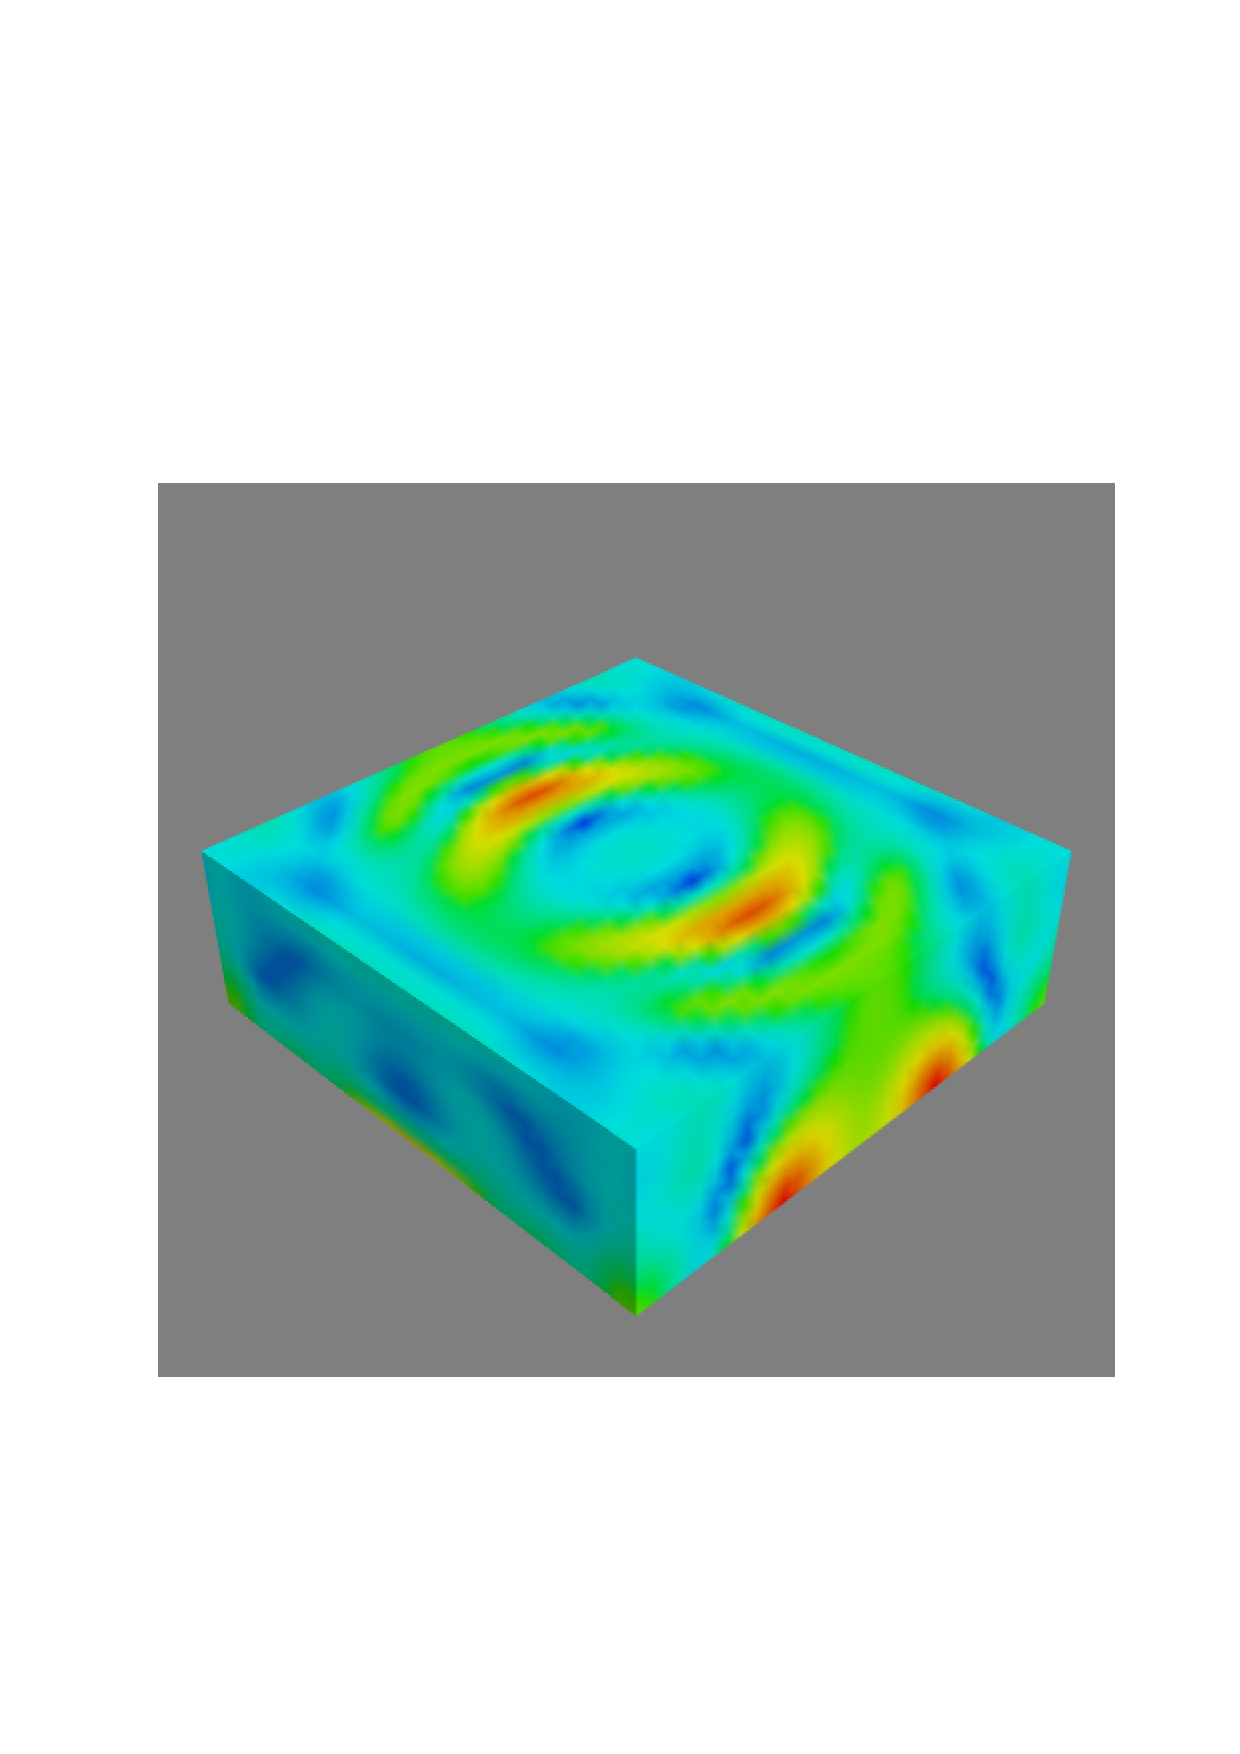
\includegraphics[width=2in]{figures/Wave28}
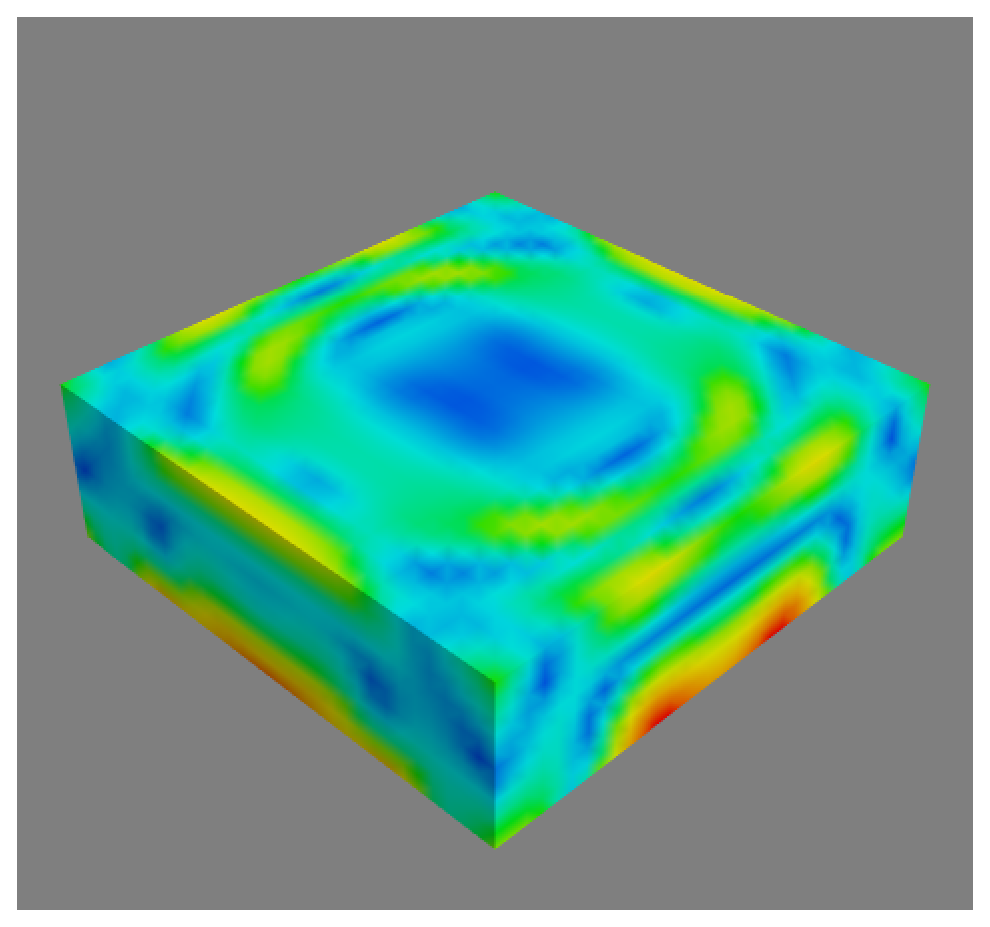
\includegraphics[width=2in]{figures/Wave32}
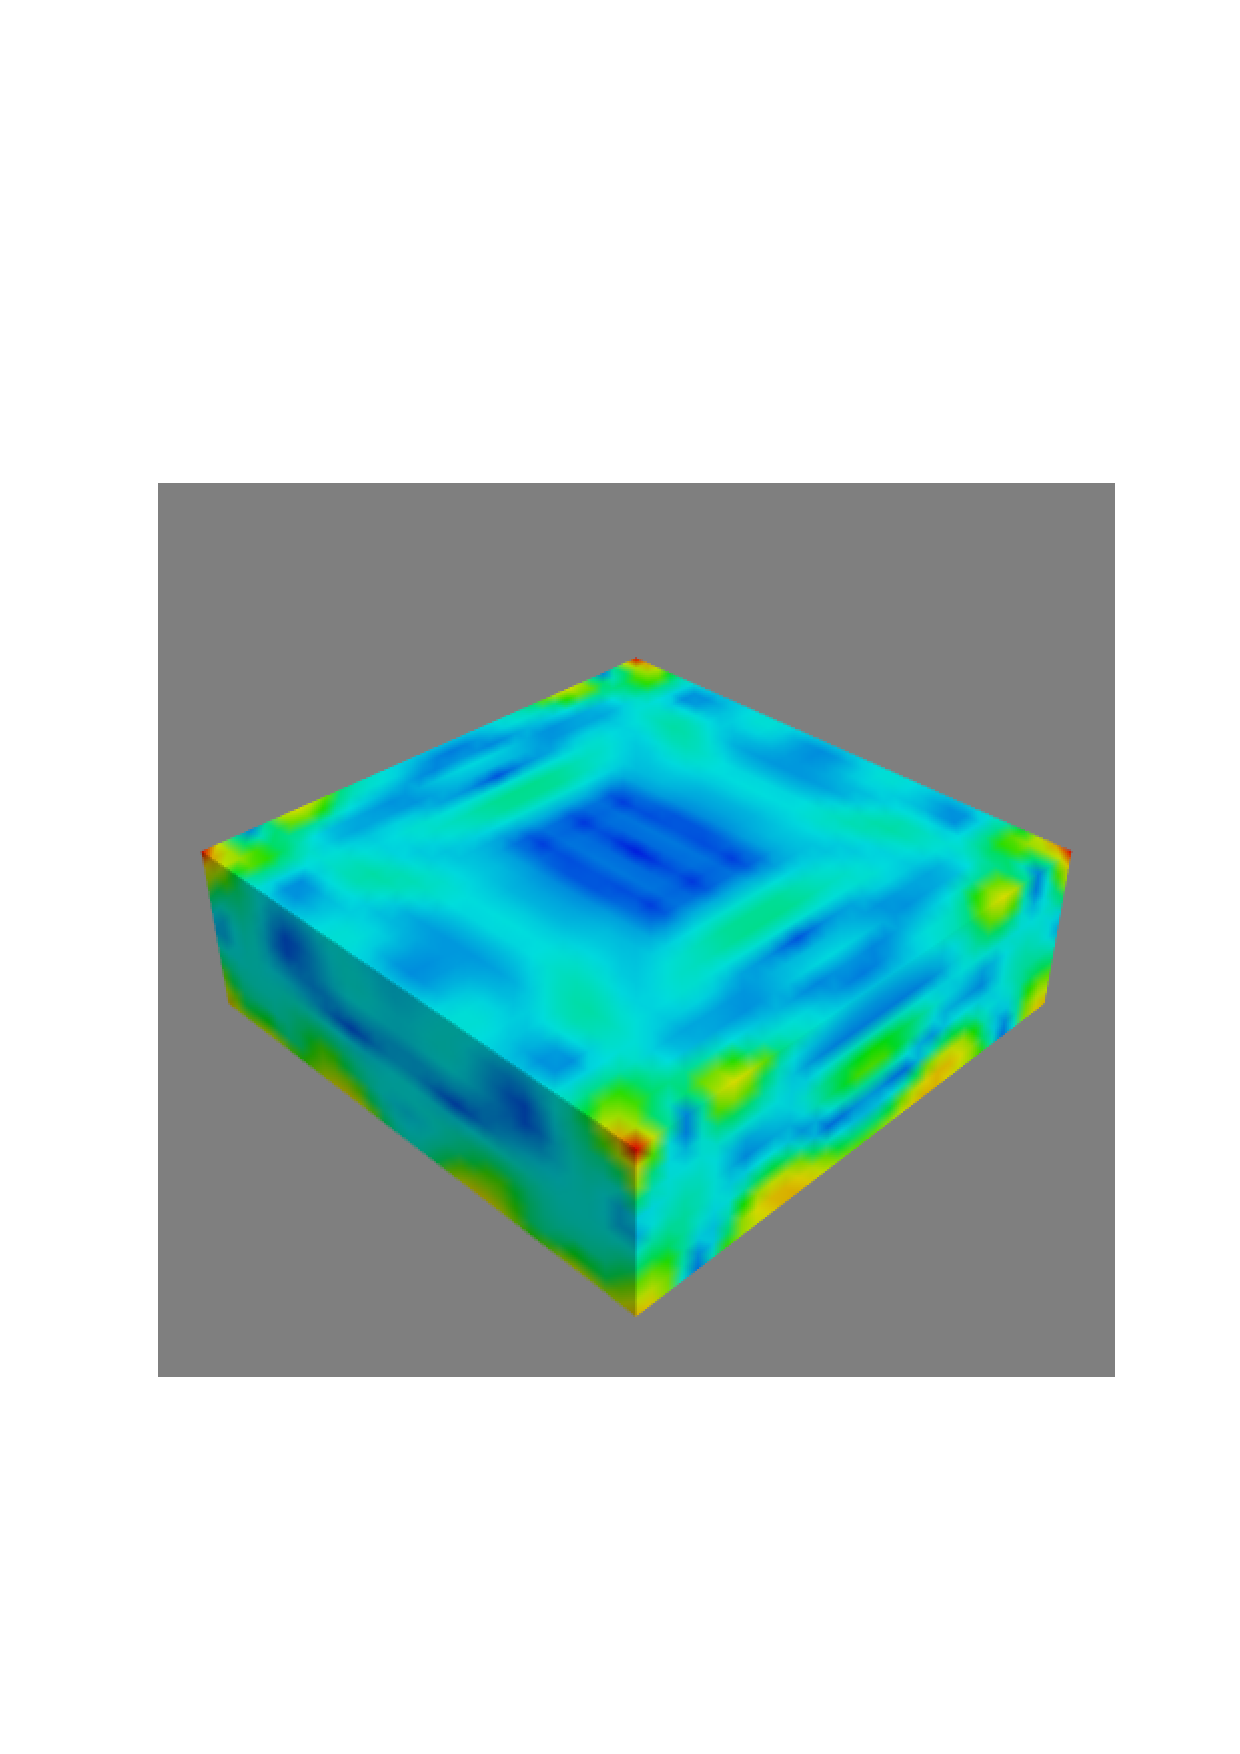
\includegraphics[width=2in]{figures/Wave36}
\end{center}
\caption{Selected time steps ($n = 11, 22, 32, 36$) of a wave propagation over a $10\mbox{km} \times 10\mbox{km} \times 3.125\mbox{km}$ block 
from a point source initially at $(5\mbox{km},5\mbox{km},0)$
with time step size $h=0.02083$. Color represents the displacement.
Here the view is oriented onto the bottom face.
\label{WAVE FIG 2}}
\end{figure}

The following script uses the \code{wavePropagation} function to solve the
wave equation for a point source located at the bottom face of a block. The width of the block in 
each direction on the bottom face is $10\mbox{km}$ ($x\hackscore 0$ and $x\hackscore 1$ directions ie. \code{l0} and \code{l1}).
The \code{ne} gives the number of elements in $x\hackscore{0}$ and $x\hackscore 1$ directions.  
The depth of the block is aligned with the $x\hackscore{2}$-direction. 
The depth (\code{l2}) of the block in
the $x\hackscore{2}$-direction is chosen so that there are 10 elements and the magnitude of the
of the depth is chosen such that the elements 
become cubic. We chose 10 for the number of elements in $x\hackscore{2}$-direction so that the 
computation would be faster. \code{Brick($n\hackscore 0,  n\hackscore 1, n\hackscore 2,l\hackscore 0,l\hackscore 1,l\hackscore 2$)} is an \finley function which creates a rectangular mesh 
with $n\hackscore 0 \times n\hackscore 1 \times n\hackscore2$ elements over the brick $[0,l\hackscore 0] \times [0,l\hackscore 1] \times [0,l\hackscore 2]$.
\begin{python}
from esys.finley import Brick
ne=32          # number of cells in x_0 and x_1 directions
width=10000.  # length in x_0 and x_1 directions
lam=3.462e9
mu=3.462e9
rho=1154.
tend=60
U0=1. # amplitude of point source
# spherical source at middle of bottom face
xc=[width/2.,width/2.,0.]
# define small radius around point xc
src_radius = 0.03*width
print "src_radius = ",src_radius
mydomain=Brick(ne,ne,10,l0=width,l1=width,l2=10.*width/32.)
h=(1./5.)*inf(sqrt(rho/(lam+2*mu))*inf(domain.getSize())
print "time step size = ",h
ts, u_pc0, u_pc1, u_pc2 =   \
                    wavePropagation(mydomain,h,tend,lam,mu,rho,xc, src_radius, U0)
\end{python}
The \function{domain.getSize()} return the local element size $\Delta x$. The 
\function{inf} makes sure that the Courant condition~\ref{WAVE dyn 66} olds everywhere in the domain. 

The script is available as \file{wave.py} in the \ExampleDirectory \index{scripts!\file{wave.py}}. 
To visualize the results from the data directory: 
\begin{verbatim} 
mayavi2 -d usoln.1.vtu -m SurfaceMap &
\end{verbatim}
You can rotate this figure by clicking on it with the mouse and moving it around.
Again use \code{Configure Data} to move backwards and forward in time, and 
also to choose the results (acceleration, displacement or $u\hackscore x$) by using \code{Select Scalar}. Figure \ref{WAVE FIG 2} shows the results for the displacement at various time steps.

\begin{figure}[t!]
\centerline{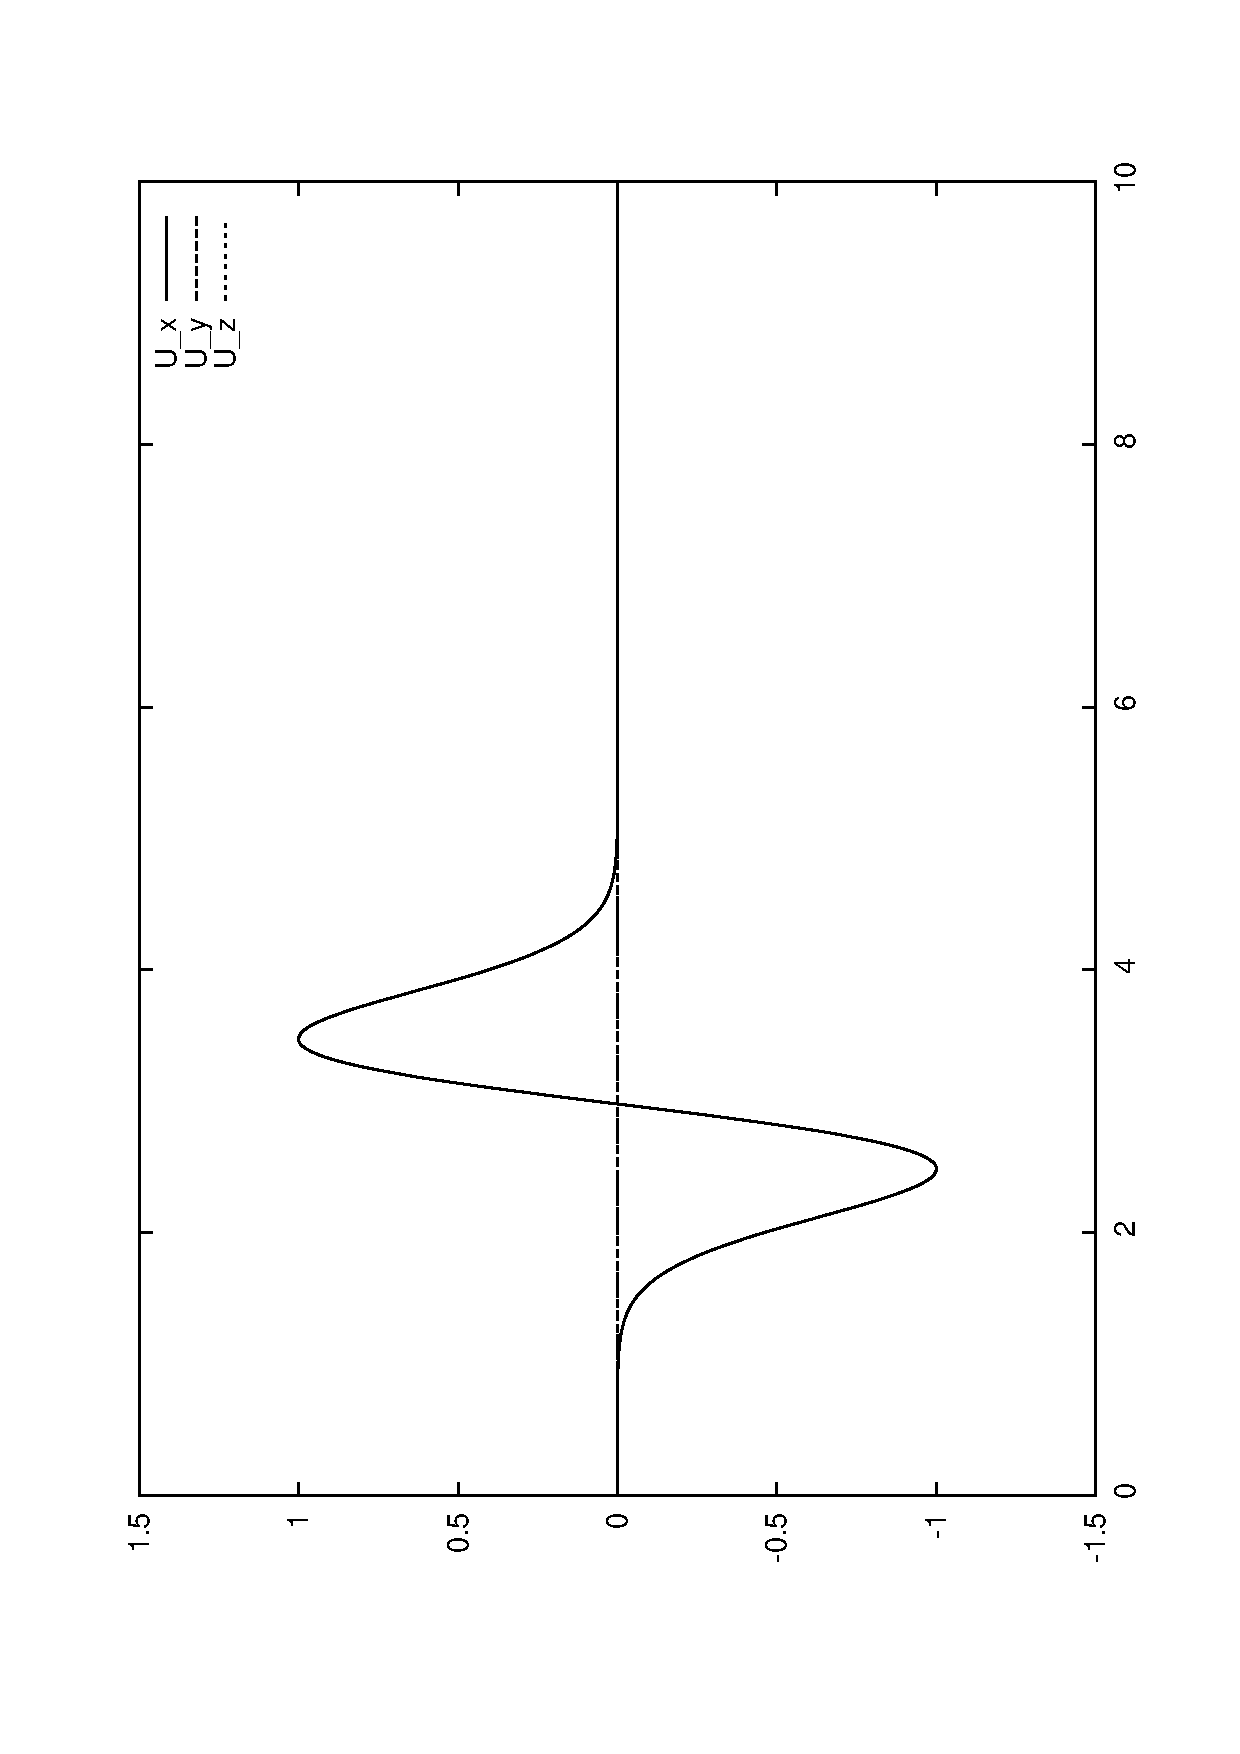
\includegraphics[width=4.in, angle=-90]{figures/WavePC}}
\caption{Amplitude at Point source from the Simulation.}
\label{WAVE FIG 1}
\end{figure}

It remains to show some possibilities to inspect the collected data \var{u_pc0}, \var{u_pc1} and \var{u_pc2}.
One way is to write the data to a file and then use an external package such as \gnuplot, excel or OpenOffice to read the data for further analysis. The following code shows one possible form to write the data to the 
file \file{./data/U_pc.out}:
\begin{python}
u_pc_data=FileWriter('./data/U_pc.out')
for i in xrange(len(ts)) :
    u_pc_data.write("%f %f %f %f\n"%(ts[i],u_pc0[i],u_pc1[i],u_pc2[i]))
u_pc_data.close()
\end{python}
The \code{U_pc.out} stores 4 columns of data: $t,u\hackscore x,u\hackscore y,u\hackscore z$ 
respectively, where $u\hackscore x,u\hackscore y,u\hackscore z$ are the $x\hackscore 0,x\hackscore 1,x\hackscore 2$ components of the displacement vector $u$ at the point source. These can be
plotted easily using any plotting package. In \gnuplot the command:
\begin{verbatim}
 plot 'U_pc.out' u 1:2 title 'U_x' w l lw 2, 'U_pc.out' u 1:3 title 'U_y' w l lw 2, 
'U_pc.out' u 1:4 title 'U_z' w l lw 2
\end{verbatim}
will reproduce Figure~\ref{WAVE FIG 1} (As expected this is identical to the input signal shown in Figure~\ref{WAVE FIG 1.2})2. It is pointed out that we are not using the
standard \PYTHON \function{open} to write to the file \code{U_pc.out} as it is not safe
when running \escript under MPI, see chapter~\ref{EXECUTION} for more details.

Alternatively, one can implement plotting the results at run time rather than in a post-processing step. This avoids
the generation of an intermediate data file. In {\it escript} the preferred way of creating 2D plots of 
time dependent data is \MATPLOTLIB. The following script creates the plot and writes it into the 
file \file{u_pc.png} in the PNG image format:
\begin{python}
import matplotlib.pyplot as plt
if getMPIRankWorld() == 0:
    plt.title("Displacement at Point Source")
    plt.plot(ts, u_pc0, '-', label="x_0", linewidth=1)
    plt.plot(ts, u_pc1, '-', label="x_1", linewidth=1)
    plt.plot(ts, u_pc2, '-', label="x_2", linewidth=1)
    plt.xlabel('time')
    plt.ylabel('displacement')
    plt.legend()
    plt.savefig('u_pc.png', format='png')
\end{python}
You can add the \function{plt.show()} to create a interactive browser window. Please not that 
through the \code{getMPIRankWorld() == 0} statement the plot is generated on one processor only (in this case the rank 0 processor) when run under MPI. 

Both options for processing the point source data are include in the example file \file{wave.py}. There other options available to process these data in particular through the \SCIPY package , eg Fourier transformations. It is beyond the scope of this users guide to document the usage of \SCIPY for time series analysis but is highly recommended that users  use \SCIPY to any further data processing.

